\scanpage{18}
\uline{NB} Donnons nous un plongement
\[k\lhook\joinrel\xrightarrow{\varphi}\mathbb C\]
\deleted{alors ce}\inserted{alors ce} plongement permet de réduire le groupe structural
du torseur $P_{X,x}$ \deleted{\unsure{sous}} \inserted{$\mathcal M_{g,\nu}$}
au sous-groupe $\mathcal G_{g,\nu}^{+}$, ou ce qui revient au même, le groupe
structural $\mathcal N_{g,\nu}$ de $Q_X$ au sous-groupe $\Gamma_{g,\nu}^{+}$
(structure de ``discrétification'' \inserted{``orientée''} du groupe profini
$\Pi_{X,x}$) : \deleted{A fortiori,}
\[
(\unsure{21})\quad\left\{\begin{array}{ccc}
P_{X,x}^{\varphi}\subset P_{X,x}&(\Leftrightarrow)&Q_X^{\varphi}\subset Q_X\\
\mathcal G_{g,\nu}^{+}\subset\mathcal M_{g,\nu}&&\Gamma_{g,\nu}^{+}\subset\mathcal N_{g,\nu}
\end{array}\right.
\]
a fortiori, prenant une adhérence, on trouve
\[
(22)\quad\left\{\begin{array}{ccc}
\widehat P_{X,x}^{\varphi}\subset P_{X,x}&\Leftrightarrow&\widehat Q_X^{\varphi}\subset Q_X\\
\widehat{\mathcal G}_{g,\nu}^{+}\subset\mathcal M_{g,\nu}&&\widehat\Gamma_{g,\nu}^{+}\subset\mathcal N_{g,\nu}
\end{array}\right.
\]
\deleted{qui}\inserted{dont} la donnée équivaut, par ce qui précède à la page précédente,
à celle d'un iso \deleted{plongt} $\widetilde{\mathbb Q}\longrightarrow\overline{\mathbb Q}$.
\unsure{\&} Cela montre que
\margin{\figure{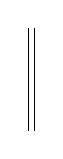
\begin{tikzpicture}\draw (0,0)--(0,1.3);\draw (.08,0)--(.08,1.3);\end{tikzpicture}}}
cette donnée (22) \unsure{ne peut en aucun cas} décrire $\varphi$ lui-même, mais seult
$\varphi|\widetilde{\mathbb Q}$.
Mais je pense que la conn. de \deleted{$\unsure{\varphi}$} $P_{X,x}^{\varphi}$
(ou $Q_X^{\varphi}$) lui-même, pour tt $X$ (et tt $g,\nu$) définit $\varphi$\ldots
\mspage{17}
